\documentclass{article}

\usepackage{iclr2026_conference,times}
\input{math_commands.tex}
\usepackage{amsmath,amssymb}
\usepackage{booktabs}
\usepackage{array}
\usepackage{enumitem}
\usepackage{graphicx}
\usepackage{microtype}
\usepackage{float}
\usepackage[section]{placeins}
\usepackage{tikz}
\usepackage{pgfplots}
\usepackage{xcolor}
\usepackage{hyperref}
\usepackage{url}
\usetikzlibrary{arrows.meta,positioning,calc,fit}
\pgfplotsset{compat=1.18}

\definecolor{cwblue}{HTML}{2F6690}
\definecolor{cwgreen}{HTML}{3A7D44}
\definecolor{cwgold}{HTML}{B7791F}
\definecolor{cwred}{HTML}{A23B3B}
\hypersetup{colorlinks=true,citecolor=cwblue,linkcolor=cwblue,urlcolor=cwblue}
\newcommand{\method}{\textsc{DoLens}}
\newcommand{\doop}{\operatorname{do}}
\newcommand{\compat}{\mathcal{C}}

\title{\method: Intervene, Measure, and Reason\\
about Causes and Counterfactuals\\
in Hidden Worlds}

\author{Anonymous authors}

% Anonymous ICLR submission.
% \iclrfinalcopy

\begin{document}
\maketitle

\begin{abstract}
Causal reasoning begins with a choice of evidence. A capable agent decides which
intervention to perform, which variables to read, and when the collected evidence
supports a causal conclusion. Current language-model evaluations primarily score
answers to supplied causal descriptions, while broad scientific environments mix
causal inference with domain scripts and long-horizon control. We introduce
\method, an executable interactive environment for active causal reasoning in
hidden finite-state causal worlds. A model receives opaque variables, a causal
query, a legal
experiment interface, and a structured terminal schema. It gathers selected joint
counts through passive observation or batched hard interventions. One exact engine
generates the feedback and verifies five terminal objects: total effects,
individual counterfactual probabilities, experimental decisions, minimal adjustment sets,
and mediator structure. Counterfactual scoring ranges over every cross-world
coupling compatible with the CPT world, so equally compatible structural causal
models receive the same legal answer set. Variable elimination and ancestral
sampling preserve the full-joint reference semantics while accelerating a 15-node sparse
benchmark by $338.4\times$ for selected marginals and $102.5\times$ for batch
feedback. The resulting environment isolates a central scientific skill: using a
controlled experiment budget to recover causal structure and effects from a hidden
mechanism.
\end{abstract}

\section{Introduction}

A causal question often arrives before the decisive data. A scientist can observe
the system, perturb a controllable variable, select a measurement panel, inspect
the outcome, and adapt the next experiment. The quality of the conclusion depends
on the whole loop. An agent that computes a correct estimand from a completed data
table exercises one part of this capability. An agent that chooses the evidence
also exercises causal search, measurement selection, and experimental economy.

Language-model causal benchmarks have made formal causal inference measurable.
CLadder constructs identifiable graph, query, and data triples, then verbalizes
the causal model and sufficient quantities for a static answer
\citep{jin2023cladder}. Causal experimental-design methods choose interventions
that inform a graph or target query \citep{toth2022active,tigas2023differentiable},
including settings where the treatment can only be perturbed indirectly
\citep{ailer2023sequential,dern2024targeted}. Scientific-agent environments add
long-horizon interaction across rich domains \citep{jansen2024discoveryworld}.
These lines establish the ingredients for a focused evaluation object: an LLM
faces a hidden causal mechanism, controls a finite experimental interface, and
receives an exact verdict on the resulting causal answer.

\method{} realizes this object with finite causal Bayesian networks. The world is
a DAG and a finite-state conditional probability table for every node. The prompt
replaces internal variable names with opaque tokens and keeps the graph, CPT
entries, truth, and scorer sealed. It exposes legal interventions, readable
variables, a maximum readout width, and the terminal JSON schema. The model can
request a passive batch or a hard intervention, together with a selected readout.
The environment returns sparse joint counts for that readout and preserves every
other variable as hidden state. Figure~\ref{fig:overview} shows the complete
method: the sealed world, the metered evidence surface, the episode loop, the
single exact engine, and the compatible-set counterfactual rule.

\begin{figure}[t]
  \centering
  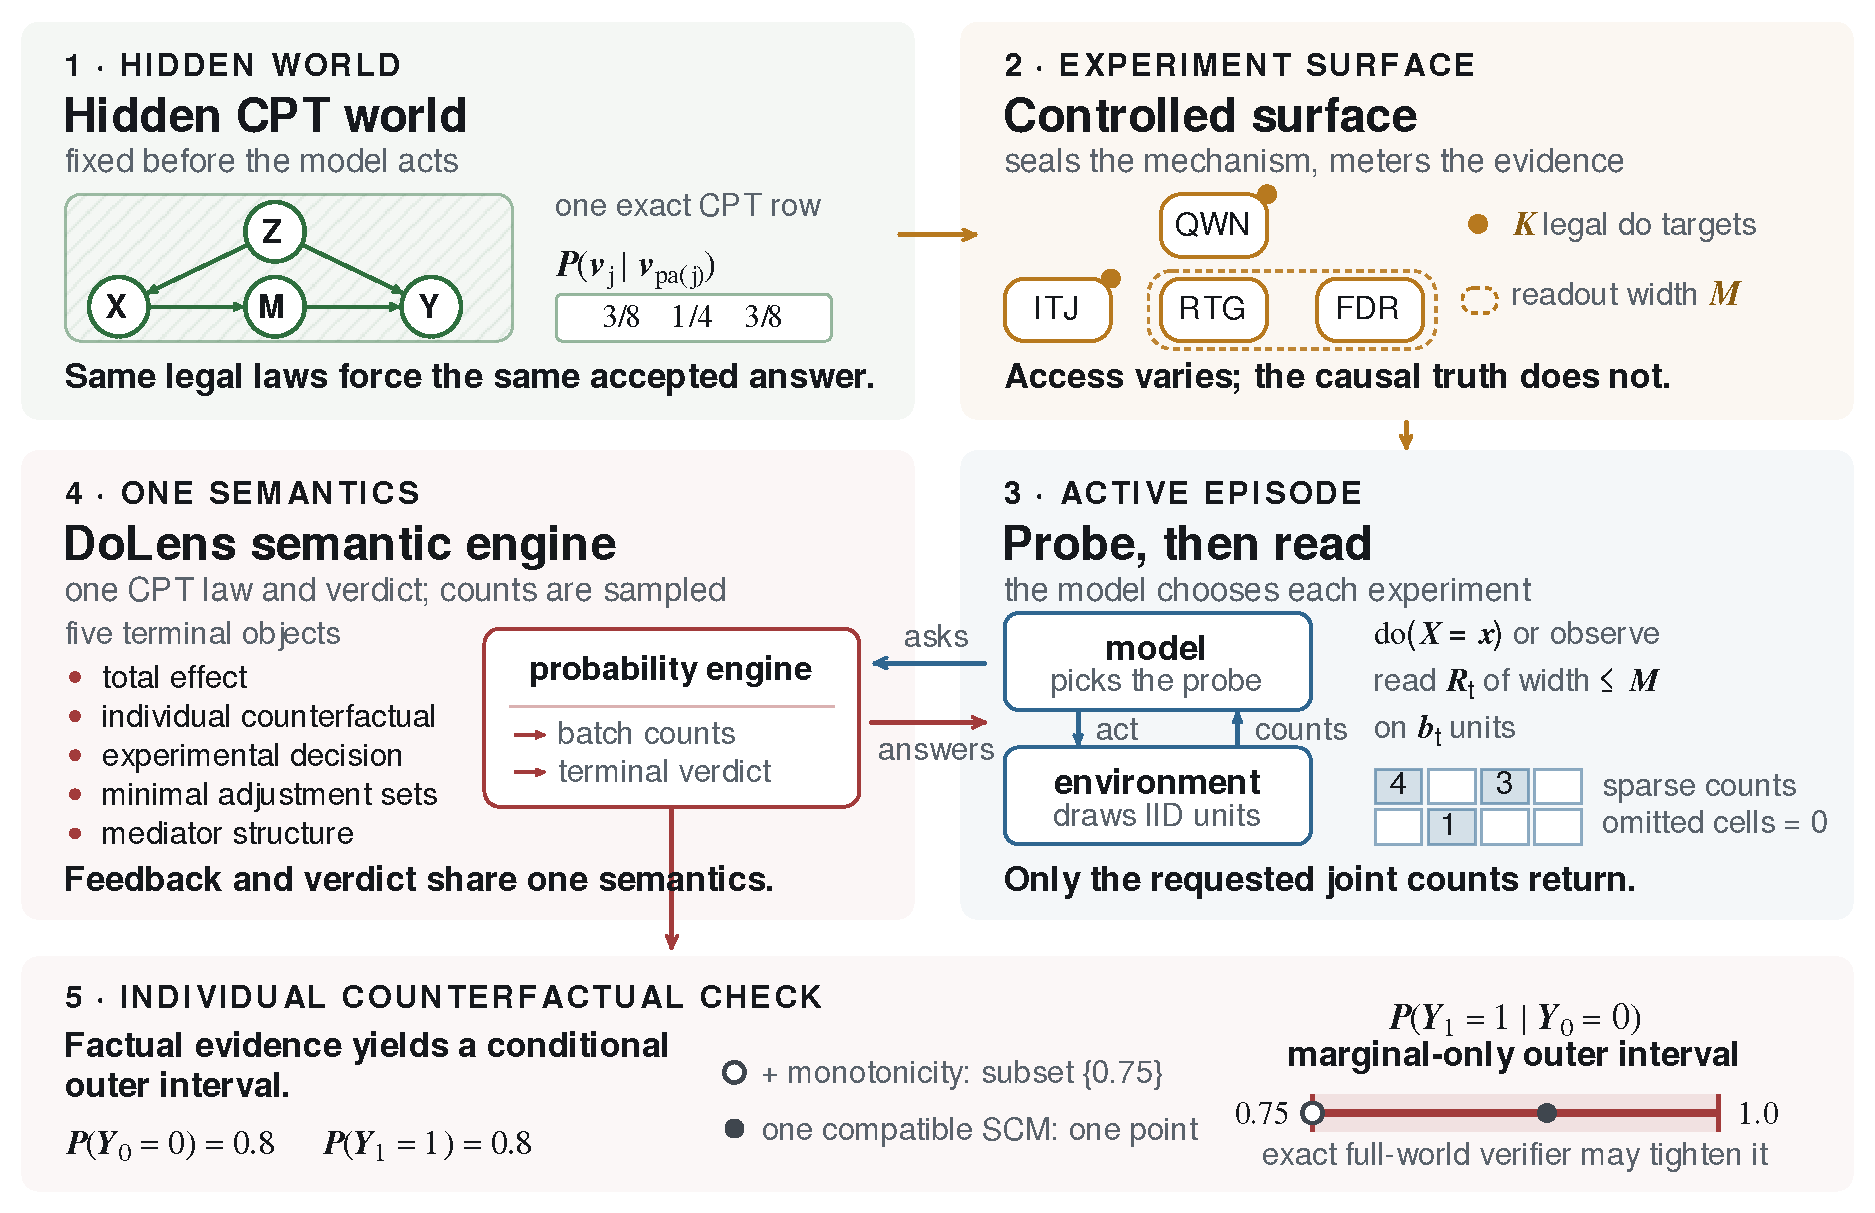
\includegraphics[width=\linewidth]{figures/overview.pdf}
  \caption{\textbf{The \method{} engine.} A hidden finite CPT world fixes one
  exact causal truth before the model acts, and worlds with identical legal laws
  must share an accepted answer. Rendering seals the mechanism and meters what
  the model may use: opaque labels, $K$ legal do targets, and readout width $M$,
  so evidence access varies while the causal truth does not. Inside that surface
  the episode is a loop in which the model chooses a perturbation and a readout
  and receives only the requested joint counts. One probability engine
  generates that feedback and verifies all five terminal objects. For
  an individual counterfactual query, assigned factual treatment and observed
  outcome define the conditioning event. Endpoint marginals supply a Fr\'echet
  outer interval for the requested probability, while the verifier computes the
  exact interval over complete mechanisms compatible with the DAG and every CPT
  row. A single SCM picks one point inside that interval, and an added
  cross-world assumption selects a smaller subset.}
  \label{fig:overview}
\end{figure}

This interaction creates a direct test of experimental causal reasoning. Consider
an ATE query whose treatment and outcome are read-only. The model must use legal
probes on other variables and decide which endpoints to measure together. A
decision query separates exploratory interventions from the final deployment
action. Discovery queries ask for minimal adjustment sets or mediator order after
the model has manipulated and observed the hidden system. The same renderer and
runtime support every task, so task variation comes from the causal query and the
interaction surface.

Counterfactual evaluation receives a second benefit from the finite CPT
representation. A CPT world fixes each interventional marginal and leaves their
cross-world coupling open.

\begin{center}
\setlength{\fboxsep}{7pt}
\fcolorbox{cwblue!55}{cwblue!4}{%
\begin{minipage}{0.92\linewidth}
\textbf{Example: factual evidence still leaves an individual probability open.}
Let $Y_x$ denote the outcome of the same unit under $\doop(X=x)$. Suppose
$P(Y_0{=}1)=0.2$ and $P(Y_1{=}1)=0.8$. In a population of 100 units, 20 would
have outcome 1 under $X=0$, while 80 would have outcome 1 under $X=1$. The
marginals leave the overlap between these groups unspecified. Now observe one
individual with $Y_0=0$ and ask for the probability that this same individual
would have $Y_1=1$. Endpoint marginals imply
\[
  P(Y_1{=}1\mid Y_0{=}0)\in[0.75,1].
\]
Both endpoints are attainable by endpoint-event couplings. Constraints from
the complete DAG and all CPT rows can tighten this outer interval. A cross-world
assumption can select a smaller subset; monotonicity $Y_1\ge Y_0$ contracts this
conditional interval to the point $0.75$.
\end{minipage}}
\end{center}

A generated SCM selects one complete compatible mechanism. Encoding that selection
as the label also encodes its cross-world preference. \method{} keeps the full
compatible mechanism set. The model submits one individual counterfactual
probability, and the hidden verifier scores its distance to the sharp compatible
interval. The task
therefore measures counterfactual reasoning supported by the stated causal
information \citep{balke1997bounds,pearl2009causality}.

The work contributes a unified experimental causal interface, a five-task
construction pipeline, and an exact scalable verifier. The construction samples a
world and query first, then samples the legal intervention subset $K$ and
observation width $M$. The verifier uses variable elimination for query marginals
and action-keyed ancestral
sampling for feedback. Differential tests match the original full-joint semantics,
and end-to-end tests exercise every task from prompt through terminal score.

\section{Related work and benchmark position}

\paragraph{Causal reasoning datasets.}
CLadder grounds natural-language questions in symbolic causal graphs, queries,
and oracle answers across association, intervention, and counterfactual levels
\citep{jin2023cladder}. Its generator supplies the causal specification and the
quantities needed for an identifiable answer. CauGym generates questions and
symbolic solutions from sampled SCMs for seven effect estimands, then repackages
them as training and stress-test sets for post-training
\citep{chen2026caugym}. These datasets evaluate whether a model can apply formal
causal rules to supplied evidence. \method{} makes evidence construction part of
the evaluated behavior: the model creates the numerical record through legal
experiments and selected measurements.

\paragraph{Causal experiment design.}
ABCI integrates posterior inference over causal models and target queries with
sequential intervention selection \citep{toth2022active}. Differentiable
multi-target design optimizes batches of target-state pairs
\citep{tigas2023differentiable}. A-ICP selects experiments that expose stable
parent sets \citep{gamella2020active}. Sequential instrument selection and
targeted indirect design address settings in which the treatment itself is
unavailable for manipulation \citep{ailer2023sequential,dern2024targeted}.
\method{} converts these experimental intuitions into a model-facing benchmark
protocol with opaque symbols, discrete tool calls, selected measurements, and
task-specific exact scoring.

\paragraph{Interactive causal and scientific agents.}
DiscoveryWorld evaluates hypothesis formation, experiment design, analysis, and
action across multimodal scientific tasks \citep{jansen2024discoveryworld}.
CausalGame asks agents to design protocols, collect data, and solve interactive
games containing selection bias, measurement error, and hidden confounding
\citep{chen2026causalgame}. CausaLab samples a hidden SCM, lets an agent
intervene on a manipulator system, and scores both held-out prediction and
recovered causal mechanisms \citep{yang2026causalab}. These environments expose
scientific agency through rich task-specific dynamics. \method{} places the same
agency inside a compact probability laboratory: every action has a precise
hard-do meaning, every readout is a selected joint distribution, and every
terminal object is checked by the same exact causal layer.

\begin{table}[H]
\centering
\scriptsize
\setlength{\tabcolsep}{2.2pt}
\begin{tabular}{
  >{\raggedright\arraybackslash}p{1.85cm}
  >{\raggedright\arraybackslash}p{2.15cm}
  >{\centering\arraybackslash}p{0.85cm}
  >{\raggedright\arraybackslash}p{1.75cm}
  >{\raggedright\arraybackslash}p{2.45cm}
  >{\raggedright\arraybackslash}p{1.55cm}
  >{\raggedright\arraybackslash}p{2.15cm}}
\toprule
Benchmark & World evidence & Probe & Returned evidence & Scored object & CF rule & Verifier \\
\midrule
CLadder & supplied model and sufficient data & -- & prompt-fixed quantities & three-rung causal answer & SCM point & causal-inference oracle \\
CauGym & supplied graph and probabilities & -- & prompt-fixed quantities & seven effect estimands & SCM point & answer and format rewards \\
DiscoveryWorld & hidden multimodal world & \checkmark & world-mediated observations & task completion and explanatory knowledge & -- & procedural task metrics \\
CausalGame & hidden game process & \checkmark & protocol-specific measurements & decision and causal report & -- & survival and rubric scores \\
CausaLab (preprint) & hidden sampled SCM & \checkmark & laboratory record schema & prediction, graph, and equations & SCM truth & task and mechanism scores \\
\textbf{\method{}} & \textbf{hidden finite CPT world} & \checkmark & \textbf{model-selected joint counts} & \textbf{five typed causal objects} & \textbf{compatible set} & \textbf{exact oracle and keyed replay} \\
\bottomrule
\end{tabular}
\caption{\textbf{Comparison with representative causal datasets and agent
benchmarks.} Probe means that the model creates evidence during the episode.
The CF column records the semantics of counterfactual labels. \method{} combines
a hidden mechanism, model-chosen perturbations, variable-level readout control,
five causal objects, compatible-set counterfactual scoring, and exact replay.}
\label{tab:position}
\end{table}

Table~\ref{tab:position} separates three capabilities that are often bundled
together. Static causal datasets measure inference from a completed record.
Interactive environments measure experiment planning inside a scientific or
game process. \method{} joins active evidence acquisition to an exact causal
benchmark substrate. The selected readout makes measurement choice an explicit
decision alongside intervention choice. The compatible-set rule assigns the same
legal counterfactual answers to every SCM coupling represented by one CPT world.
Action-keyed sampling then makes stochastic histories reproducible under symbol
permutation, batch partition, and interleaved actions.

\section{The \method{} episode}

\subsection{A hidden finite causal world}

A world is $W=(G,\Theta)$, where $G$ is a finite DAG and $\Theta$ contains one
exact categorical CPT row for every parent assignment. For variables
$V_1,\ldots,V_n$ in topological order,
\begin{equation}
  P_W(v_1,\ldots,v_n)
  = \prod_{j=1}^{n} P_{\Theta_j}(v_j\mid v_{\mathrm{pa}(j)}).
  \label{eq:factorization}
\end{equation}
Hard intervention $\doop(V_j=x)$ replaces the mechanism for $V_j$ with a point
mass at $x$. This gives one semantic owner for passive and interventional data
\citep{pearl2009causality,peters2017elements}.

The renderer samples opaque three-letter labels and public state tokens. The
model receives variable domains, the query, legal hard-do targets, readable
variables, legal batch sizes, and the terminal schema. Graph edges, CPT values,
internal names, task truth, and scorer state remain sealed.

\subsection{Action, measurement, and feedback}

An experiment is a compact triple
\begin{equation}
  a_t=\left(
    \underbrace{\doop(X=x)\ \text{or}\ \mathrm{observe}}_{\text{perturb}},
    \underbrace{R_t}_{\text{read}},
    \underbrace{b_t}_{\text{repeat}}
  \right),
  \qquad |R_t|\le M.
  \label{eq:action}
\end{equation}
The intervention target belongs to a seed-owned legal set of size $K$. The
readout $R_t$ is a nonempty subset of readable variables and excludes the active
intervention target. The environment draws $b_t$ IID units from the same hidden
world and reports
\begin{equation}
  C_{R_t}\sim\mathrm{Multinomial}
  \left(b_t,\underbrace{P_W(R_t\mid\doop(X=x))}_{\text{selected law}}\right).
  \label{eq:feedback}
\end{equation}
Only nonzero cells appear in the JSON count map. This sparse representation keeps
feedback proportional to the batch and selected domain, while preserving an exact
meaning for every omitted cell.

\subsection{Sampling the interaction surface}

The construction order separates causal content from evidence access. It samples
a legal world, a query anchor, and an exact task answer, then draws $K$ and $M$.
The optional answerability diagnostic remains separate from generation and does
not filter or label the five task families. Conditional on the eligible intervention variables, the width
$K$ is uniform and the subset is uniform at that width. The readout width $M$ is
sampled independently from $1$ through $n$. A fixed world and query can therefore
appear with narrow or broad evidence access while retaining the same causal truth.

\section{One engine, five causal tasks}

Table~\ref{tab:tasks} summarizes the implemented tasks. Each task returns one
structured terminal object. The exact owner computes its truth from the sealed
world, and the public protocol uses visible labels throughout.

\begin{table}[H]
\centering
\footnotesize
\setlength{\tabcolsep}{3.5pt}
\renewcommand{\arraystretch}{1.08}
\begin{tabular}{>{\raggedright\arraybackslash}p{3.55cm}>
                {\raggedright\arraybackslash}p{2.65cm}>
                {\raggedright\arraybackslash}p{2.35cm}>
                {\raggedright\arraybackslash}p{3.05cm}}
\toprule
Task & Question & Terminal object & Experimental separation \\
\midrule
\textbf{Total effect} & Effect of $X$ on $Y$ & scalar ATE & $X,Y$ read-only; probe legal non-endpoints \\
\cmidrule(lr){1-4}
\textbf{Individual counterfactual} & Same individual's outcome under another treatment, given factual evidence & scalar probability & query endpoints read-only \\
\cmidrule(lr){1-4}
\textbf{Experimental decision} & Deployment value optimizing an outcome event & target-value intervention & deployment variable read-only during evidence collection \\
\cmidrule(lr){1-4}
\textbf{Backdoor adjustment} & Covariates that block every backdoor path & all minimal sets & manipulate and read candidate covariates \\
\cmidrule(lr){1-4}
\textbf{Mediator structure} & Variables and consecutive edges on directed $X\to Y$ paths & mediator set and order & perturb path candidates and read descendants \\
\bottomrule
\end{tabular}
\caption{\textbf{Five tasks share one interaction loop.} The separation column
states how each task assigns distinct roles to evidence actions and the terminal
causal object.}
\label{tab:tasks}
\end{table}

\subsection{Effects and individual counterfactuals}

For treatment states $x_1,x_0$ and outcome event $Y=y$, the total-effect target
is
\begin{equation}
  \tau=P_W(Y=y\mid\doop(X=x_1))-P_W(Y=y\mid\doop(X=x_0)).
  \label{eq:ate}
\end{equation}
The generic interaction keeps $X$ and $Y$ read-only, turning the query into an
indirect experimental problem. Passive batches and interventions on legal
non-endpoints provide the evidence.

For assigned factual treatment $x_f$, observed factual outcome $y_f$,
counterfactual treatment $x_c$, and target outcome $y^\star$, the model predicts
$q=P(Y_{x_c}=y^\star\mid Y_{x_f}=y_f)$. The world induces a compatible set of
nonparametric SCMs $\compat(W)$, and the hidden verifier computes
\begin{equation}
  [L,U]=\left[
  \inf_{\mathcal M\in\compat(W)} q(\mathcal M),
  \sup_{\mathcal M\in\compat(W)} q(\mathcal M)
  \right]
  \quad\text{\scriptsize(all compatible complete mechanisms)}.
  \label{eq:cfset}
\end{equation}
Let $p_f=P(Y=y_f\mid\doop(X=x_f))$ and
$p_c=P(Y=y^\star\mid\doop(X=x_c))$. Their Fr\'echet outer interval is
$[\max(0,p_f+p_c-1)/p_f,\min(p_f,p_c)/p_f]$. The exact verifier retains all
complete mechanisms compatible with the DAG and every CPT row, so its sharp
interval is contained in that outer interval and can be strictly tighter. The
model returns one scalar in $[0,1]$; the scorer reports membership and continuous
distance to the exact interval.

\subsection{Decision and structural discovery}

The experimental-decision task names a deployment variable $D$, an outcome event,
and a minimize or maximize objective. Evidence actions operate on separate legal
targets. The terminal answer chooses one value of $D$, and the verifier reports
exact regret against every deployment value. This separation evaluates whether
the model can use experiments to support a later action.

The two discovery tasks return causal structure relevant to a named query.
Backdoor adjustment returns the full family of inclusion-minimal sets. Mediator
discovery returns each variable on a directed treatment-outcome path and every
consecutive path edge. Set precision, recall, F1, and exact match preserve partial
credit while the exact-match fields retain a strict structural verdict.

\section{Exact and reproducible execution}

\subsection{One probability semantics, two execution paths}

Full-joint enumeration remains the reference oracle. Selected marginals use
factor elimination with the same CPT rows and mechanism replacement.
For maximum domain size $d$, induced width $w$, and selected width $m$, its cost
is $O(nd^{w+1}+d^m)$. The selected law therefore avoids materializing $d^n$
assignments whenever the graph permits a narrow elimination order.

Interactive feedback uses ancestral sampling. Each unit visits the nodes once in
topological order and samples from the active CPT row, giving $O(bnd)$ time for a
batch of size $b$. The output map stores at most $\min(b,d^m)$ occupied cells.

\subsection{Action-keyed outcome tapes}

Every random draw is addressed by a versioned key containing the canonical
intervention, sample index, and node. Visible labels, requested readout, batch
partition, and action interleaving stay outside this address. The same causal
experiment therefore receives the same latent units when a renderer permutes
symbols or a policy divides one batch into several calls. This common-randomness
contract supports paired model comparisons and exact replay.

\section{Validation}

\subsection{Semantic tests}

Table~\ref{tab:validation} records the validation layers. Exact differential tests
compare selected variable elimination with full-joint enumeration over random
multi-valued worlds, natural distributions, and hard interventions under the
shared numerical contract. Ancestral
sampling tests compare every nonzero assignment interval with the full-joint law.
Protocol tests cover strict visible labels, selected projection, sparse counts,
budget updates, tape invariance, and terminal parsing. The complete suite executes
103 tests: 102 pass and one optional test is skipped; both Ruff checks pass.

\begin{table}[H]
\centering
\small
\setlength{\tabcolsep}{5pt}
\begin{tabular}{>{\raggedright\arraybackslash}p{3.2cm}>
                {\raggedright\arraybackslash}p{5.35cm}>
                {\raggedright\arraybackslash}p{2.55cm}}
\toprule
Layer & Test & Result \\
\midrule
Selected inference & 24 random multi-valued worlds under natural and hard-do laws & matches full-joint reference \\
Batch semantics & 12 random DAGs, every nonzero assignment interval & identical categorical mass \\
Reproducibility & rename, projection, split-batch, and interleaved actions & invariant tape draws \\
Task loop & prompt, batch feedback, terminal parser, exact scorer & all five modes execute \\
Repository suite & unit tests, lint, and format & 102 pass; 1 skipped; checks clean \\
\bottomrule
\end{tabular}
\caption{\textbf{Validation targets semantic ownership.} Each accelerated or
interactive component is compared with the exact reference law or a deterministic
protocol invariant.}
\label{tab:validation}
\end{table}

\subsection{End-to-end task demonstration}

The runtime demonstration samples one instance per task, renders its opaque prompt,
executes a legal selected-measure intervention, returns sparse counts, and sends an
exact terminal object through the public parser and scorer. A representative ATE
episode exposes variables \texttt{ITJ}, \texttt{RTG}, and \texttt{FDR}; keeps the
first two read-only; and permits intervention on \texttt{FDR}. The command
\begin{center}
\small\ttfamily
\{ "type":"intervene", "target":"FDR", "value":"state\_1",\\
\hspace{1.2cm}"measure":["RTG","ITJ"], "batch\_size":8 \}
\end{center}
returns three occupied joint-count cells totaling eight samples. The terminal ATE
is then checked against the exact value $316/479$. The other four modes traverse
the same state machine and return their own typed terminal objects.

\subsection{Scaling the exact verifier}

Figure~\ref{fig:speedup} compares the accelerated paths with the original
full-joint implementation on sparse binary chains. Every timed marginal first
passes exact Fraction equality. At 10 nodes, variable elimination is $13.8\times$
faster and ancestral feedback is $7.3\times$ faster. At 15 nodes, the speedups
reach $338.4\times$ and $102.5\times$. The growth reflects the shift from the
joint state count $2^n$ to graph width for exact queries and to $bnd$ work for
sampled feedback.

\begin{figure}[H]
  \centering
  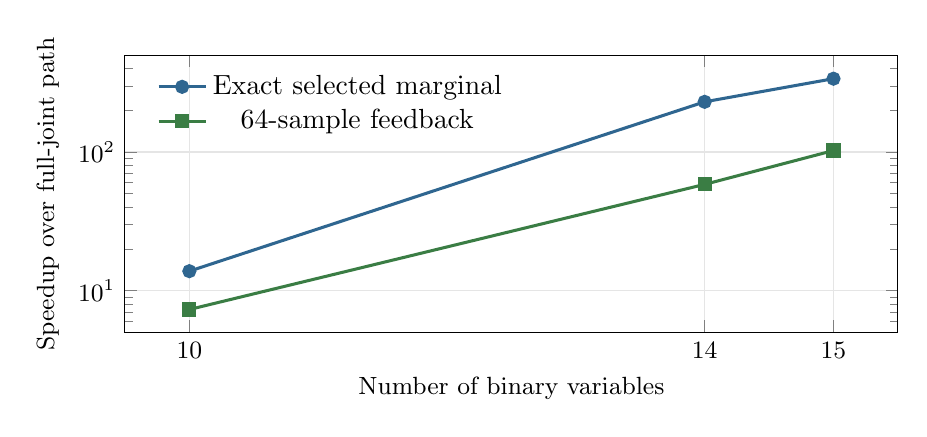
\begin{tikzpicture}
\begin{axis}[
  width=0.94\linewidth,
  height=5.1cm,
  ymode=log,
  log basis y=10,
  xlabel={Number of binary variables},
  ylabel={Speedup over full-joint path},
  xtick={10,14,15},
  ymin=5,
  ymax=500,
  grid=major,
  grid style={black!10},
  legend style={draw=none, fill=none, at={(0.03,0.97)}, anchor=north west},
  tick label style={font=\small},
  label style={font=\small},
]
\addplot[color=cwblue, mark=*, line width=1.1pt] coordinates {
  (10,13.8) (14,230.4) (15,338.4)
};
\addlegendentry{Exact selected marginal}
\addplot[color=cwgreen, mark=square*, line width=1.1pt] coordinates {
  (10,7.3) (14,58.4) (15,102.5)
};
\addlegendentry{64-sample feedback}
\end{axis}
\end{tikzpicture}


  \caption{\textbf{Query and interactive acceleration.} Median speedup over the
  full-joint reference on sparse binary chains. The exact marginal curve uses
  variable elimination; the feedback curve generates 64 IID units with ancestral
  sampling.}
  \label{fig:speedup}
\end{figure}

\section{Conclusion}

\method{} defines causal reasoning as an experiment-and-answer loop inside a
hidden finite world. The model controls interventions and measurements through a
compact JSON interface; the environment returns only selected evidence; and one
exact semantic layer verifies five causal objects. Compatible-SCM counterfactual
sets keep evaluation aligned with the causal information supplied by the world.
Exact acceleration and action-keyed replay make the same construction practical
for benchmark generation, model evaluation, and training trajectories. This
turns finite CPT worlds into an executable laboratory for measuring how models
acquire and use causal evidence.

\bibliography{references}
\bibliographystyle{iclr2026_conference}

\newpage
\appendix

\section{Formal world semantics}

Let each node $V_j$ have domain $\{0,\ldots,d_j-1\}$. The parent tuple follows a
fixed order, so every CPT row has a canonical index. A hard intervention map
$I=\{j\mapsto x_j\}$ induces
\begin{equation}
P_W(v\mid\doop(I))=
\prod_{j\notin I}P_{\Theta_j}(v_j\mid v_{\mathrm{pa}(j)})
\prod_{j\in I}\mathbf{1}[v_j=x_j].
\end{equation}
Generated worlds store CPT probabilities in float64 after one validity check and
row normalization. Fixed fixtures may instead use exact rational rows. Natural
observation is the special case $I=\varnothing$.

The public surface contains a visible permutation $\sigma$ of node labels, a
manipulability mask, a readability mask, and observation width $M$. Parsing maps
visible tokens back to canonical indices before executing any probability
operation. Feedback maps selected indices back through $\sigma$ and serializes
only nonzero cells.

\section{Task truth and diagnostics}

\subsection{Total effect}

For the rendered treatment values $x_1,x_0$ and outcome state $y$, the truth owner
evaluates Eq.~\ref{eq:ate} with exact projected interventional marginals. The
terminal diagnostics are absolute and squared error.

\subsection{Individual counterfactual probability}

Define $A=\mathbf{1}[Y_{x_c}=y^\star]$ and
$B=\mathbf{1}[Y_{x_f}=y_f]$. The CPT world fixes
$P(A=1)=p_c$ and $P(B=1)=p_f$. The requested probability is
$q=P(A=1\mid B=1)$. The two endpoint marginals alone give the Fr\'echet outer
bounds
\begin{equation}
\frac{\max(0,p_f+p_c-1)}{p_f}\le q\le
\frac{\min(p_f,p_c)}{p_f}.
\end{equation}
The truth owner optimizes the joint numerator over complete mechanisms compatible
with the DAG and every CPT row, then divides by the fixed positive factual mass
$p_f$. The model returns a scalar probability. The scorer reports membership and
distance to the resulting exact interval.

\subsection{Experimental decision}

For deployment variable $D$, admissible states $\mathcal D$, outcome event
$Y=y$, and objective $s\in\{\min,\max\}$, the oracle enumerates
$P(Y=y\mid\doop(D=d))$ for $d\in\mathcal D$. Every optimal state receives zero
regret. The scorer computes the exact gap between the chosen probability and the
objective optimum.

\subsection{Backdoor adjustment}

The structural oracle enumerates observed node sets that satisfy the backdoor
criterion for the named treatment and outcome, then retains inclusion-minimal
sets. The scorer treats the family of minimal sets as the prediction universe and
reports precision, recall, F1, and exact family match.

\subsection{Mediator structure}

The oracle enumerates directed treatment-outcome paths. The mediator set is the
union of internal path nodes. The order relation contains each consecutive edge
on at least one such path. Mediator and edge sets receive separate precision,
recall, F1, and exact-match diagnostics.

\section{Exact variable elimination}

For a requested marginal $R$, each CPT becomes a factor over one node and its
parents. A hard intervention replaces the corresponding factor with a point mass.
The engine eliminates non-readout variables in a min-fill order and multiplies the
remaining factors before canonical normalization. With induced width $w$, maximum
domain size $d$, and readout width $m$, the upper cost is
$O(nd^{w+1}+d^m)$ time. The reference implementation enumerates every assignment
and remains available for differential testing.

\section{Ancestral sampling and replay}

For each sample index $i$ and canonical node $j$, the tape produces a rational
uniform draw addressed by
\begin{equation}
  \mathrm{key}=(\mathrm{version},\mathrm{tape\ id},I,i,j).
\end{equation}
The sampler visits nodes in topological order, uses intervention values for nodes
in $I$, and inverse-samples the active CPT row for every other node. It projects
the full latent assignment to the requested readout only after the sample is
complete. A batch split preserves the same sample indices. An interleaved action
uses an independent intervention arm address.

The old full-joint batch path costs $O((n+b)d^n)$ time and
$O(d^n+d^m)$ memory. The ancestral path costs $O(bnd)$ time and
$O(n+\min(b,d^m))$ working and output memory.

\section{Construction pipeline}

The implemented generator follows this order:
\begin{enumerate}[leftmargin=1.6em,itemsep=2pt]
  \item sample a node count from the configured support;
  \item sample each finite domain size, a topological order, and a forward-edge
        subset;
  \item sample continuous float64 CPT parameters and finalize each row;
  \item enumerate legal query anchors and construct exact task truth;
  \item sample the legal intervention subset $K$ and readout width $M$;
  \item sample opaque labels and render the visible episode.
\end{enumerate}
The reference configuration samples node counts uniformly from every integer in
$\{3,\ldots,15\}$ and domains of two through five states. The scaling benchmark
uses sparse binary chains from 10 through 15 nodes.

The optional family-level answerability diagnostic uses an exact response
signature and is not applied to task generation or admission. Two candidate
worlds share a signature when every legal passive and hard-do projected
distribution is equal on the complete family surface. Effect and structural
tasks require equal answers inside each signature class. Decision tasks require a shared zero-regret
deployment action. $K$ and $M$ are sampled after this partition.

\section{Model-visible protocol}

The initial message follows a fixed shape:
\begin{quote}\small\ttfamily\raggedright
DOLENS HIDDEN-MECHANISM TASK\\
Variables and finite states: [opaque labels and state tokens]\\
Query: [typed causal question]\\
Legal experimental do targets: [visible labels]\\
measure must be a nonempty subset of readable variables\\
At most M variables may be measured per batch\\
To finish, return exactly one typed JSON object
\end{quote}

An intervention command is
\begin{quote}\small\ttfamily\raggedright
\{ "type":"intervene", "target":"LAB",\\
"value":"state\_i", "measure":["LAB", ...], "batch\_size":n \}.
\end{quote}
A passive command replaces the target and value fields with
\texttt{"type":"observe"}. The parser rejects hidden internal labels,
noncanonical state tokens, duplicate JSON keys, illegal targets, duplicate or
unreadable measurements, target-in-measure requests, and unsupported batch sizes.

\section{Validation and benchmark setup}

The marginal differential covers 24 random multi-valued worlds, both the natural
law and hard interventions, and compares every projected cell with the full-joint
reference under the shared numeric representation. Exact \texttt{Fraction}
fixtures retain equality checks. The ancestral test covers 12 random DAGs and checks the
cumulative interval assigned to every nonzero full assignment. Runtime tests cover
selected joint projection, sparse serialization, passive observation, hard-do
replacement, budget state, terminal dispatch, and all five query modes.

The acceleration benchmark uses a binary chain. The root is Bernoulli $1/2$ and
each transition preserves the parent state with probability $3/4$. Both paths
compute the last-node marginal under $\doop(V_0=1)$. The batch comparison uses 64
samples and the same action-keyed tape. Each exact timing run first checks equality
with the full-joint reference.

\end{document}
